% Figure: Sorry elimination over time
\begin{figure}[t]
\centering
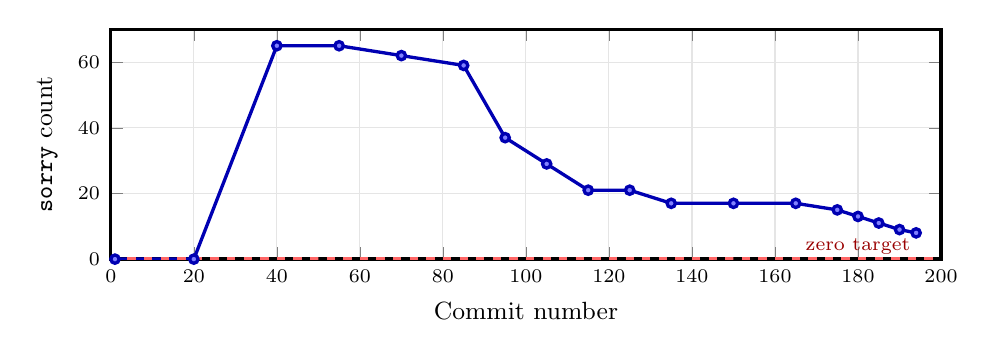
\begin{tikzpicture}
\begin{axis}[
  width=\columnwidth,
  height=4.5cm,
  xlabel={Commit number},
  ylabel={\texttt{sorry} count},
  xmin=0, xmax=200,
  ymin=0, ymax=70,
  grid=major,
  grid style={gray!20},
  line width=1.2pt,
  mark size=1.5pt,
  xlabel style={font=\small},
  ylabel style={font=\small},
  tick label style={font=\scriptsize},
  legend style={font=\scriptsize, at={(0.97,0.97)}, anchor=north east},
]
% Data points: (commit#, sorry count)
% Reconstructed from git history and session logs
\addplot[blue!70!black, mark=*, mark options={fill=blue!50}] coordinates {
  (1, 0)    % initial commit, no proofs yet
  (20, 0)   % building infrastructure
  (40, 65)  % proof files added with sorry placeholders
  (55, 65)  % infrastructure phase
  (70, 62)  % first sorry eliminated (swap, gcd)
  (85, 59)  % batch eliminations begin
  (95, 37)  % big batch: 16 sorry eliminated
  (105, 29) % 8 sorry in RBExt
  (115, 21) % more batches
  (125, 21) % model-race begins
  (135, 17) % model-race + manual proofs
  (150, 17) % infrastructure work
  (165, 17) % start of latest session
  (175, 15) % TASK-0231 partial
  (180, 13) % pq_swap + rb_push_for_drain
  (185, 11) % bubble_up + insert
  (190, 9)  % rb_count_above/below
  (194, 8)  % pq_insert dynCom (current committed)
};
\addplot[red!60, dashed, domain=0:200] {0};
\node[font=\scriptsize, text=red!60!black] at (axis cs:180,4) {zero target};
\end{axis}
\end{tikzpicture}
\caption{Sorry elimination over 194 commits. The plateau at 17 reflects
hard sorry blocked by kernel depth limits; the final descent was enabled
by the anonymous-constructor workaround (Section~3.5).}
\label{fig:sorry-timeline}
\end{figure}
